In section 2.2.1 categories of medical smart phone apps were defined. Apps in the same categories might have a similar feature set and capabilities. An app in the \textit{Alert / First Response} category might have a database that stores important contacts in the user’s area and a user interface that allows the user to quickly alert a contact in an emergency situation. An app in the \textit{Learning / Educational / Reference} category might be modelled as a quiz app which presents the user with a question and several possible answers to choose from. Answers from several questions will can be evaluated and a score is presented to the user at the end of a session. The app would be implemented with a database of questions and weighted answers, as well as an interface that presents the questions to the user sequentially.

One of the goals of this project is to define requirements for an app that provides a risk assessment of a lesion being benign or malignant. A high level description of the primary functionality of the app is the following:

\begin{itemize}[label={}]
\item The smart phone app allows the user to capture and analyse an image of a skin lesion and provide a risk assessment to the user of the lesion being a malignant melanoma.

\end{itemize}

The user might also like to save the image and results in oder to be able to compare it with other assessments in the future, or to review the assessment with a dermatologist. For comparison it might be useful to save associated metadata, such as the date and location on the body of the lesion. For convenience it might be nice to send the assessment and image via email to a specialist for review.
Secondary functionality can be described as follows:

\begin{itemize}[label={}]
\item The app allows the user to save or archive the image and corresponding assessment for future comparison and review.

\item The user can add, edit, and save metadata associated with the image of the lesion.
\item The user can browse archived images, assessments, and associated metadata.
\item The user can send a set of images with associated assessment and metadata via email.

\end{itemize}

From this high level description some basic assumptions about the app’s architecture can already be made. The app will require access to a database that can store information about an image, results of the analysis, and metadata. The app will require a user interface that allows a user to browse and edit data associated with an image. The app requires access to the smart phone’s camera api in order to capture images.

In order to formally elicit the requirements the hight level description will be broken down into structured use cases. A set of requirements will be extracted from the use cases.

\section{Use Cases}
In order to capture the formal use cases we will use a schema based on the one defined in Requirement Engineering Fundamentals \cite{9781937538774}.


\begin{table}[H]
    \begin{tabular}{ | >{\bfseries}l | p{8.35cm} |}
    \hline
    ID &  Unique designation of the use case \\ \hline
    Name & Unique name of the use case \\ \hline
    Priority & Importance of the use case according to applied prioritization technique \\ \hline
    Description &  Use case in user story form\\ \hline
    Dependencies & dependencies \\ \hline
    Trigger event & Name of the event that triggers this use case \\ \hline
    Actors & List of all the actors involved in this use case \\ \hline
    Preconditions & List of all necessary constraints that must be met before this use case can begin execution \\ \hline
    Posconditions & List of all states the system can be in immediately after the execution of the main scenario  \\ \hline
    Result & Description of the results that are produced during the use case execution \\ \hline
    Main scenario & Sequnce of events that occur during the use case. \\ \hline
    Alternate scenarios & Alternative sequence of events that might occur. \\ \hline

    Comments & Other infos \\ \hline
    \end{tabular}

    \caption{Use Case Template}
    \label{fig:uc_template}
\end{table}

\begin{table}[H]
    \begin{tabular}{ | >{\bfseries}l | p{9.5cm} |}
    \hline
    ID
    &  UC-1 \\ \hline
    Name
    & Capture Image \\ \hline
    Description
    &  As a user I can capture an image of the skin lesion that I would like to have analysed. \\ \hline
    Dependencies
    & None \\ \hline
    Trigger
    & The user activated the application and selected the "image capture" navigation item. \\ \hline
    Preconditions
    & The system state which must be active before the Use Case can occur \\ \hline
    Normal Flow
    &

    \begin{description}[align=left]
    \item [1.]Point the camera at the skin lesion.
    \item [2.]Rotate and move the camera until the skin lesion is centered and optimally sized.
    \item [3.]The user touches the screen to capture the image.
    \item [4.]The user is notified ( beep ) that the image has been captured
    \item [5.]The user can repeat from the begining
    \end{description}

    \\ \hline
    Alternate Flow & None \\ \hline
    Results
    & The captured images are placed by the system in a processing queue to calculate the lesion's border. \\ \hline
    Comments
    & It is important that a user can capture the image with just one hand. If a lesion is located on a user's hand or arm, it's not possible to use two hands. \\ \hline
    \end{tabular}

    \caption{Use Case 1}
    \label{fig:uc_1}
\end{table}
\begin{table}[H]
    \begin{tabular}{ | >{\bfseries}l | p{9.5cm} |}
    \hline
    ID
    &  UC-2 \\ \hline
    Name
    & Confirm correct calculation of skin lesion's border \\ \hline
    Description
    &  As a user I want to confirm that the skin lesion's borders have been properly calculated. \\ \hline
    Dependencies
    & UC-1 \\ \hline
    Trigger
    & The user selected the "confirm border" navigation item. \\ \hline
    Preconditions
    & At least one image has been queued for border calculation. \\ \hline
    Normal Flow
    &
    \begin{description}[align=left]
    \item [1.]The user is presented with a list of images.
    \item [2.]The following step is repeated for each image in the list.
    \item [3.]The user confirms that the border of the lesion has been precisely calculated.
    \end{description}
    \\ \hline
    Alternate Flow
    &
    \begin{description}[align=left]
    \item [A1.] Border calculation for image has not completed.
    \item [A1.3] The user can refresh the image preview until the results of the border are visible.
    \item [A1.4] The user confirms that the border of the lesion has been precisely calculated.
    \end{description}
    \begin{description}[align=left]
    \item [A2] Border calculation is not precise or has failed.
    \item [A2.3] The user confirms that the border of the lesion has not been precisely calculated.
    \item [A2.4] The image is deleted.
    \end{description}
    \\ \hline
    Results
    & After positiv confirmation, images are placed by the system in the risk assessment calculation queue.
If no images can be positively confirmed, the user can recapture new images ( UC-1 ) \\ \hline
    Comments
    & It is important that a user can capture the image with just one hand. If a lesion is located on a user's hand or arm, it's not possible to use two hands. \\ \hline
    \end{tabular}

    \caption{Use Case 2}
    \label{fig:uc_2}
\end{table}
\begin{table}[H]
    \begin{tabular}{ | >{\bfseries}l | p{9.5cm} |}
    \hline
    ID
    &  UC-3 \\ \hline
    Name
    & View risk assessment \\ \hline
    Description
    &  As a user I want to view the results of the risk assessment calculation. \\ \hline
    Dependencies
    & UC-2 \\ \hline
    Trigger
    & The user selected the "risk assessment results" navigation item. \\ \hline
    Preconditions
    & The system was able to complete the risk assessment calculation \\ \hline
    Normal Flow
    &
    \begin{description}[align=left]
    \item [1.]The user is presented with a list of images.
    \item [2.]The following step is repeated for each image in the list.
    \item [3.]The user can select and view and image and corresponding results in detail.
    \end{description}
    \\ \hline
    Alternate Flow
    &
    \begin{description}[align=left]
    \item [A1.] Risk assessment calculation for image has not completed.
    \item [A1.3] The user can refresh the results details until the results of a risk assessment is available.
    \end{description}

    \\ \hline
    Results
    &  \\ \hline
    Comments
    &  \\ \hline
    \end{tabular}

    \caption{Use Case 3}
    \label{fig:uc_3}
\end{table}
\section{Section Title}
\begin{table}[H]
    \begin{tabular}{ | >{\bfseries}l | p{9.5cm} |}
    \hline
    ID
    &  UC-5 \\ \hline
    Name
    & View archived images and data. \\ \hline
    Description
    &  As a user I want to view previously saved images and the corresponding risk assessment data. \\ \hline
    Dependencies
    & UC-4 \\ \hline
    Trigger
    & The user selects the "archive" navigation item. \\ \hline
    Preconditions
    & The system was able to complete the risk assessment calculation. \\ \hline
    Normal Flow
    &
    \begin{description}[align=left]
    \item [1.]The user is presented with a list of archived packages.
    \item [2.]The user can select an item in the list
    \item [3.]The user is presented with the images, corresponding risk assessment data and metadata for the selected item.
    \end{description}
    \\ \hline
    Alternate Flow
    &

    \\ \hline
    Results
    &
    A package of images and corresponding risk assessment data is stored in the archive with some metadata (title and comment).
    \\ \hline
    Comments
    &  \\ \hline
    \end{tabular}

    \caption{Use Case 5}
    \label{fig:uc_5}
\end{table}
\begin{table}[H]
    \begin{tabular}{ | >{\bfseries}l | p{9.5cm} |}
    \hline
    ID
    &  UC-6 \\ \hline
    Name
    & Send results to dermatologist. \\ \hline
    Description
    &  As a user I want to send a previously saved image, feature extraction data and assessment results to a dermatologist. \\ \hline
    Dependencies
    & UC-4 \\ \hline
    Trigger
    & The user selects the "archive" navigation item. \\ \hline
    Preconditions
    & The system was able to complete the risk assessment calculation. \\ \hline
    Normal Flow
    &
    \begin{description}[align=left]
    \item [1.]The user is presented with a list of archived packages.
    \item [2.]The user can select an item in the list
    \item [3.]The user can send the item as an email attachment.
    \end{description}
    \\ \hline
    Alternate Flow
    &

    \\ \hline
    Results
    &
    \\ \hline
    Comments
    &  \\ \hline
    \end{tabular}

    \caption{Use Case 6}
    \label{fig:uc_6}
\end{table}



\section{User Interface}
\begin{figure}[H]
\centering
    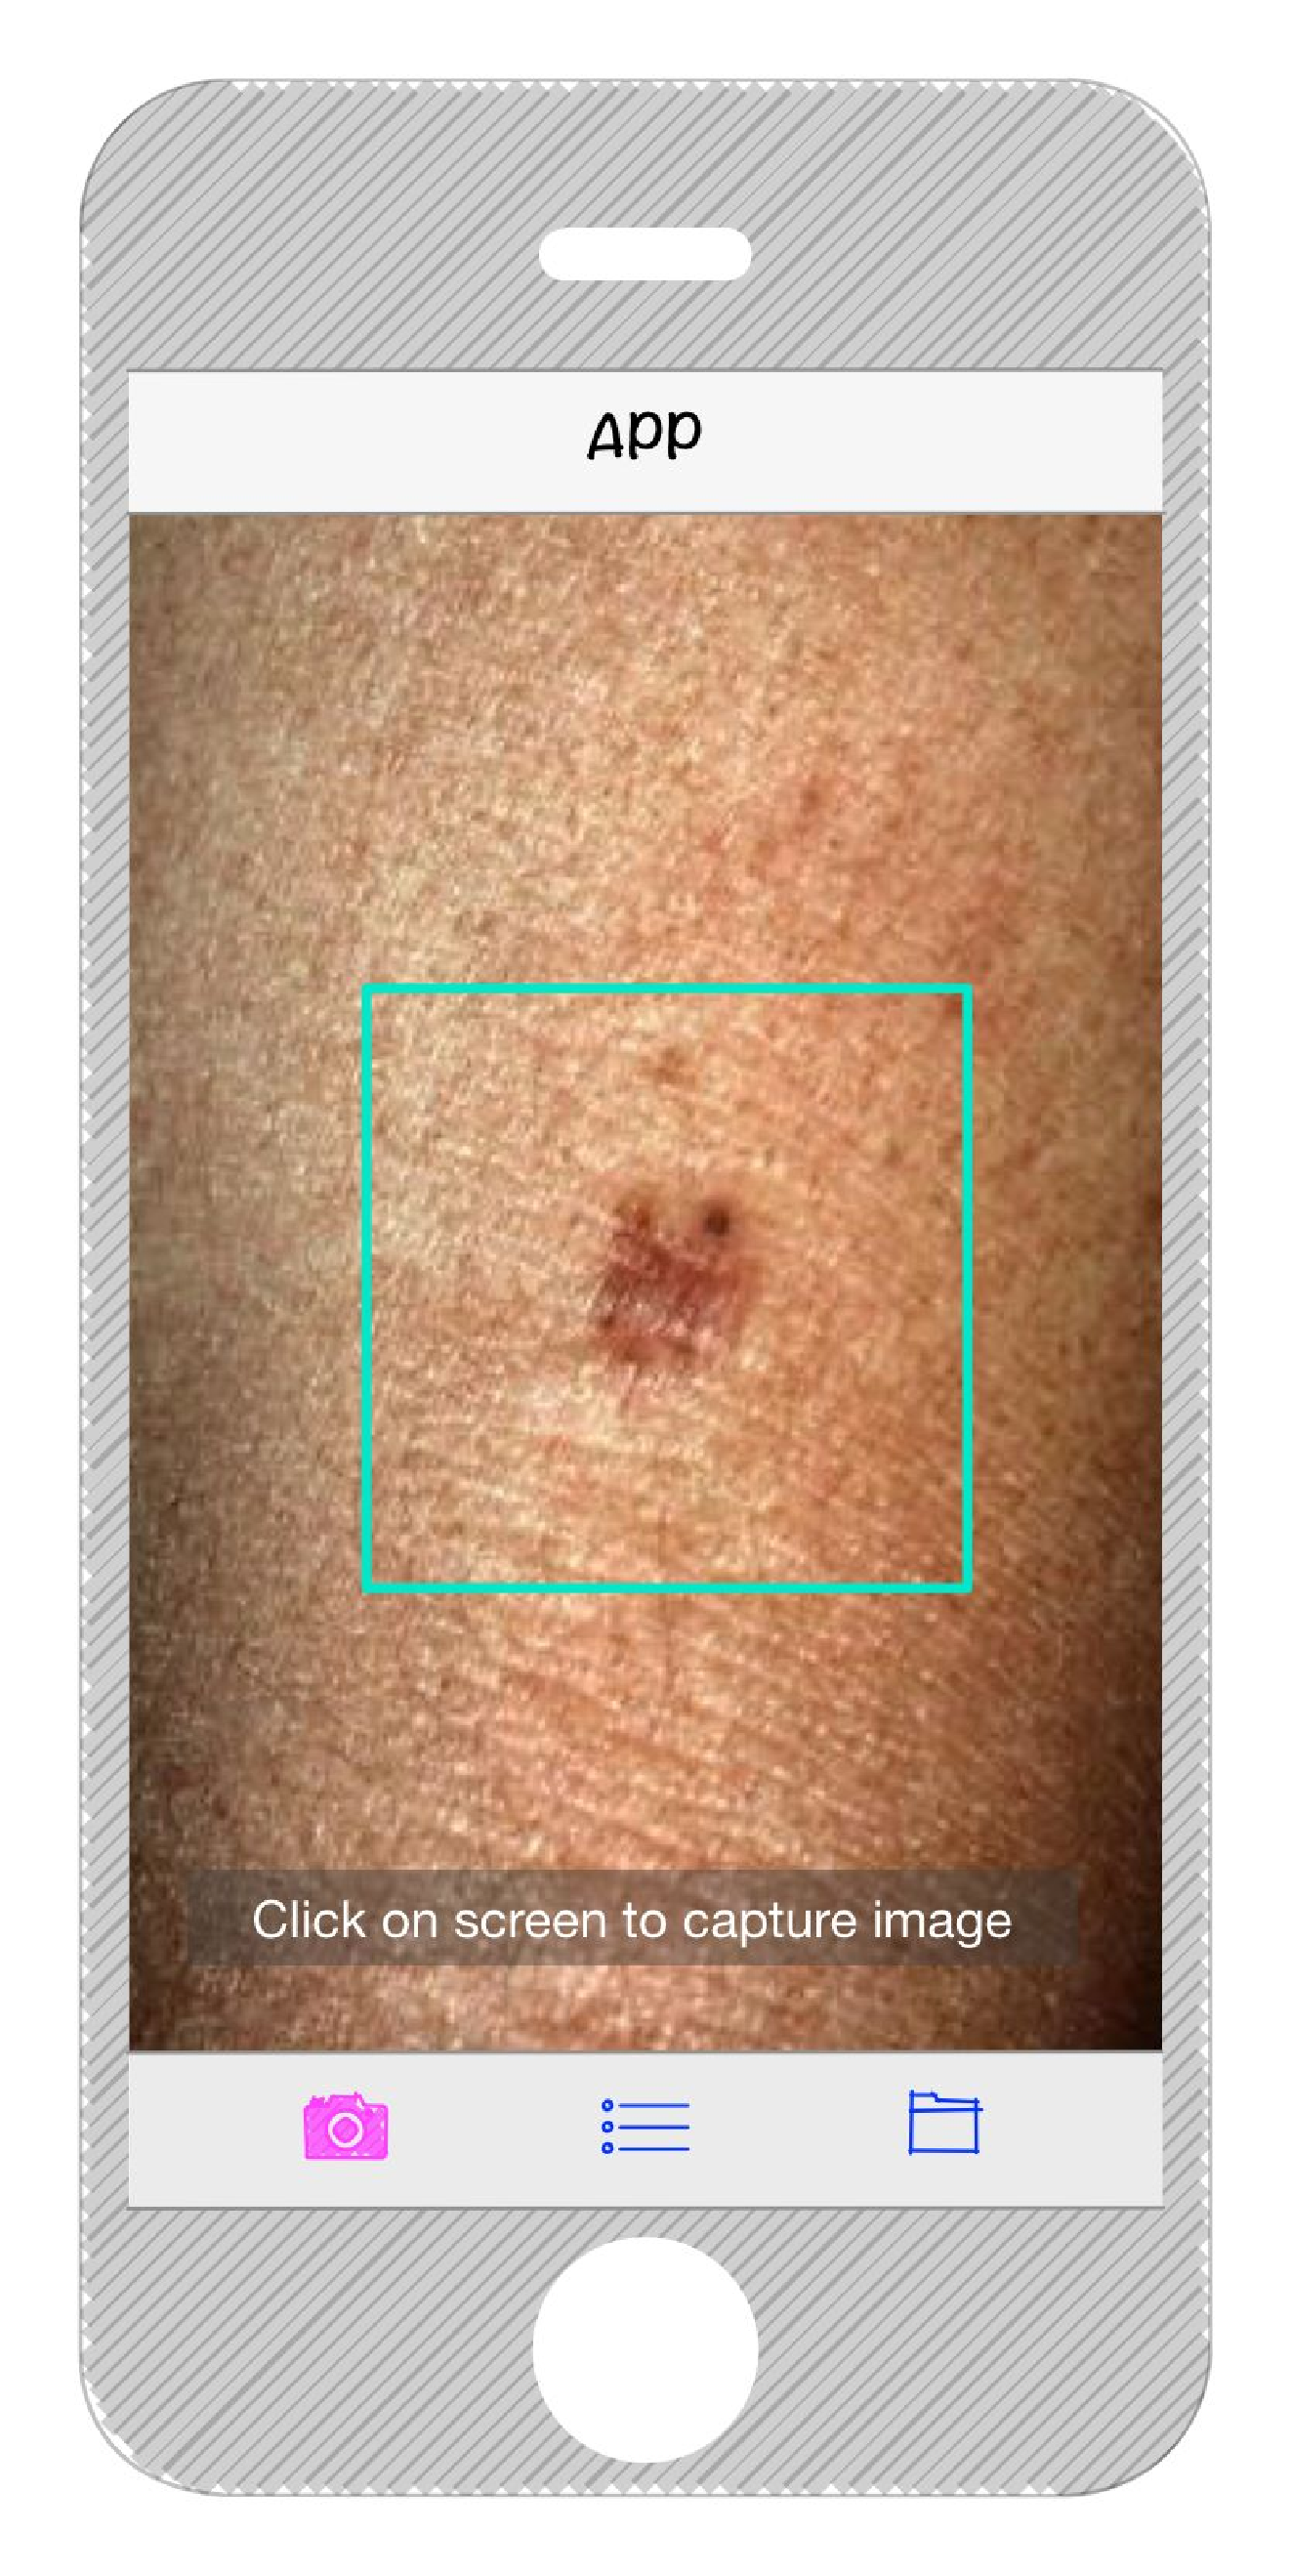
\includegraphics[height=10cm,keepaspectratio]{assets/GUI/image_capture.pdf}
    \caption{Image Capture View}
    \label{fig:image_capture}
\end{figure}

\begin{figure}[H]
    \centering
    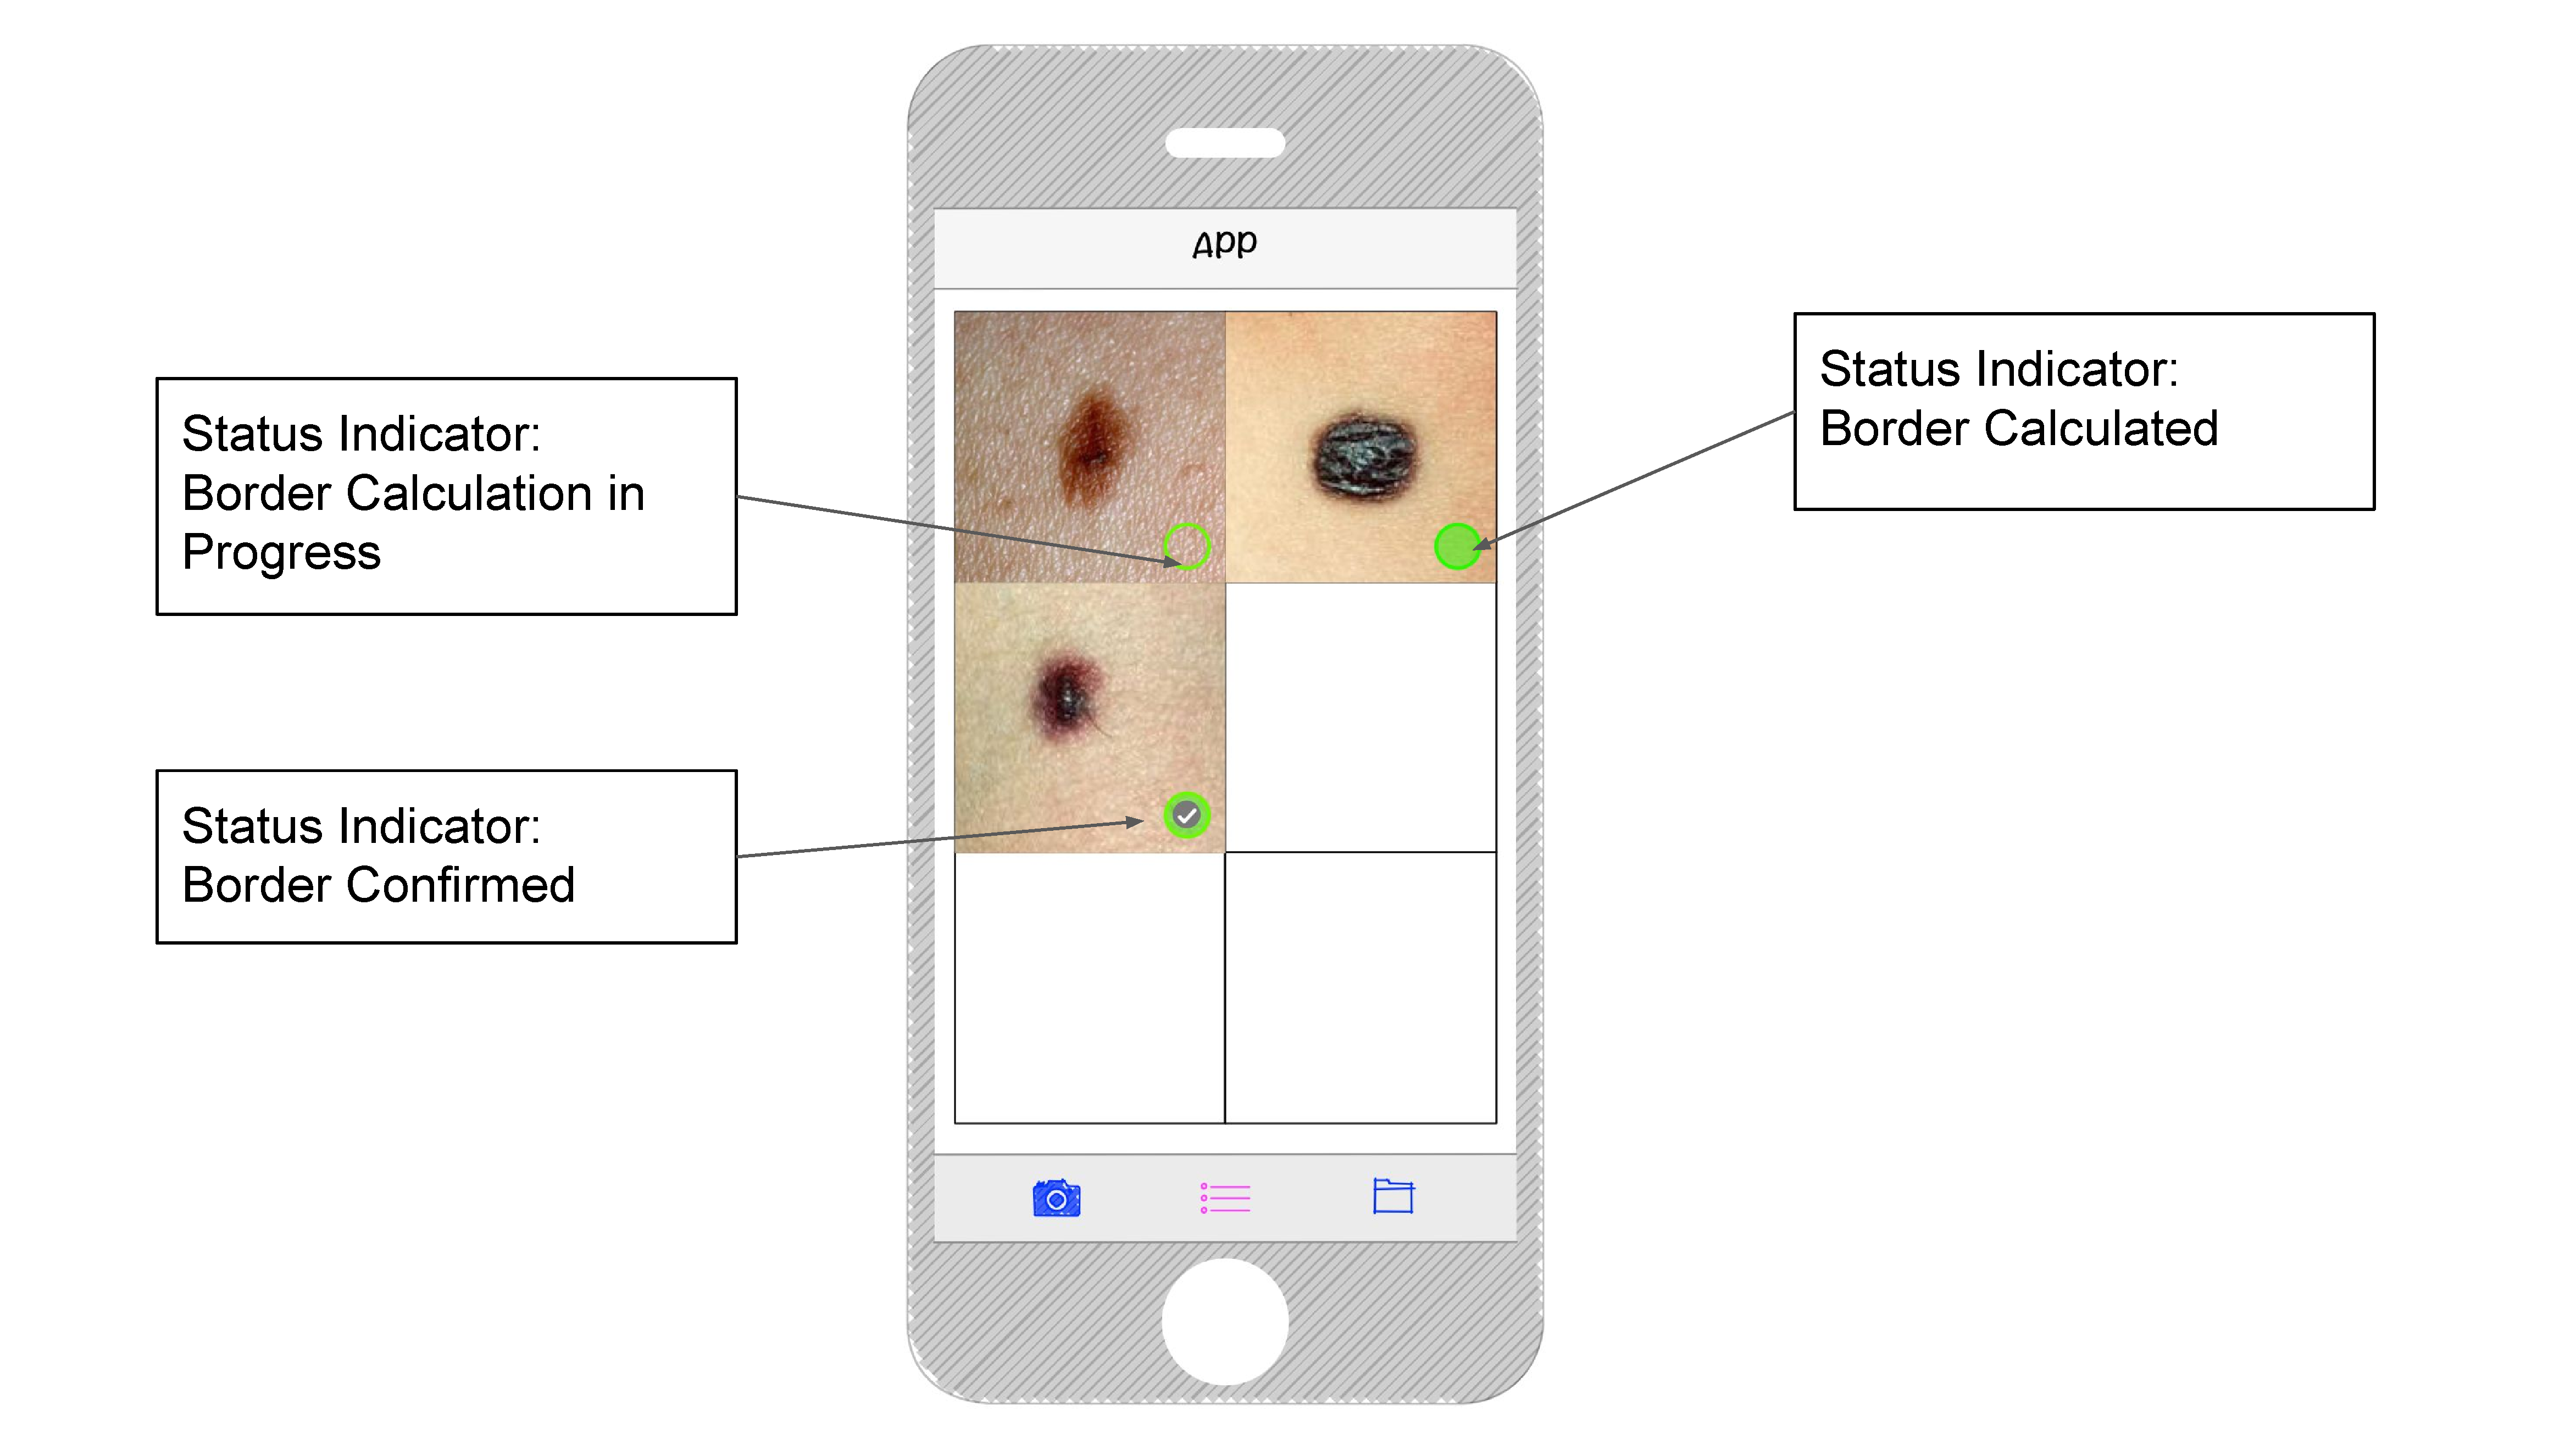
\includegraphics[height=10cm,keepaspectratio]{assets/GUI/image_list_view.pdf}
    \caption{Image List View}
    \label{fig:image_list_view}
\end{figure}

\begin{figure}[H]
    \centering
    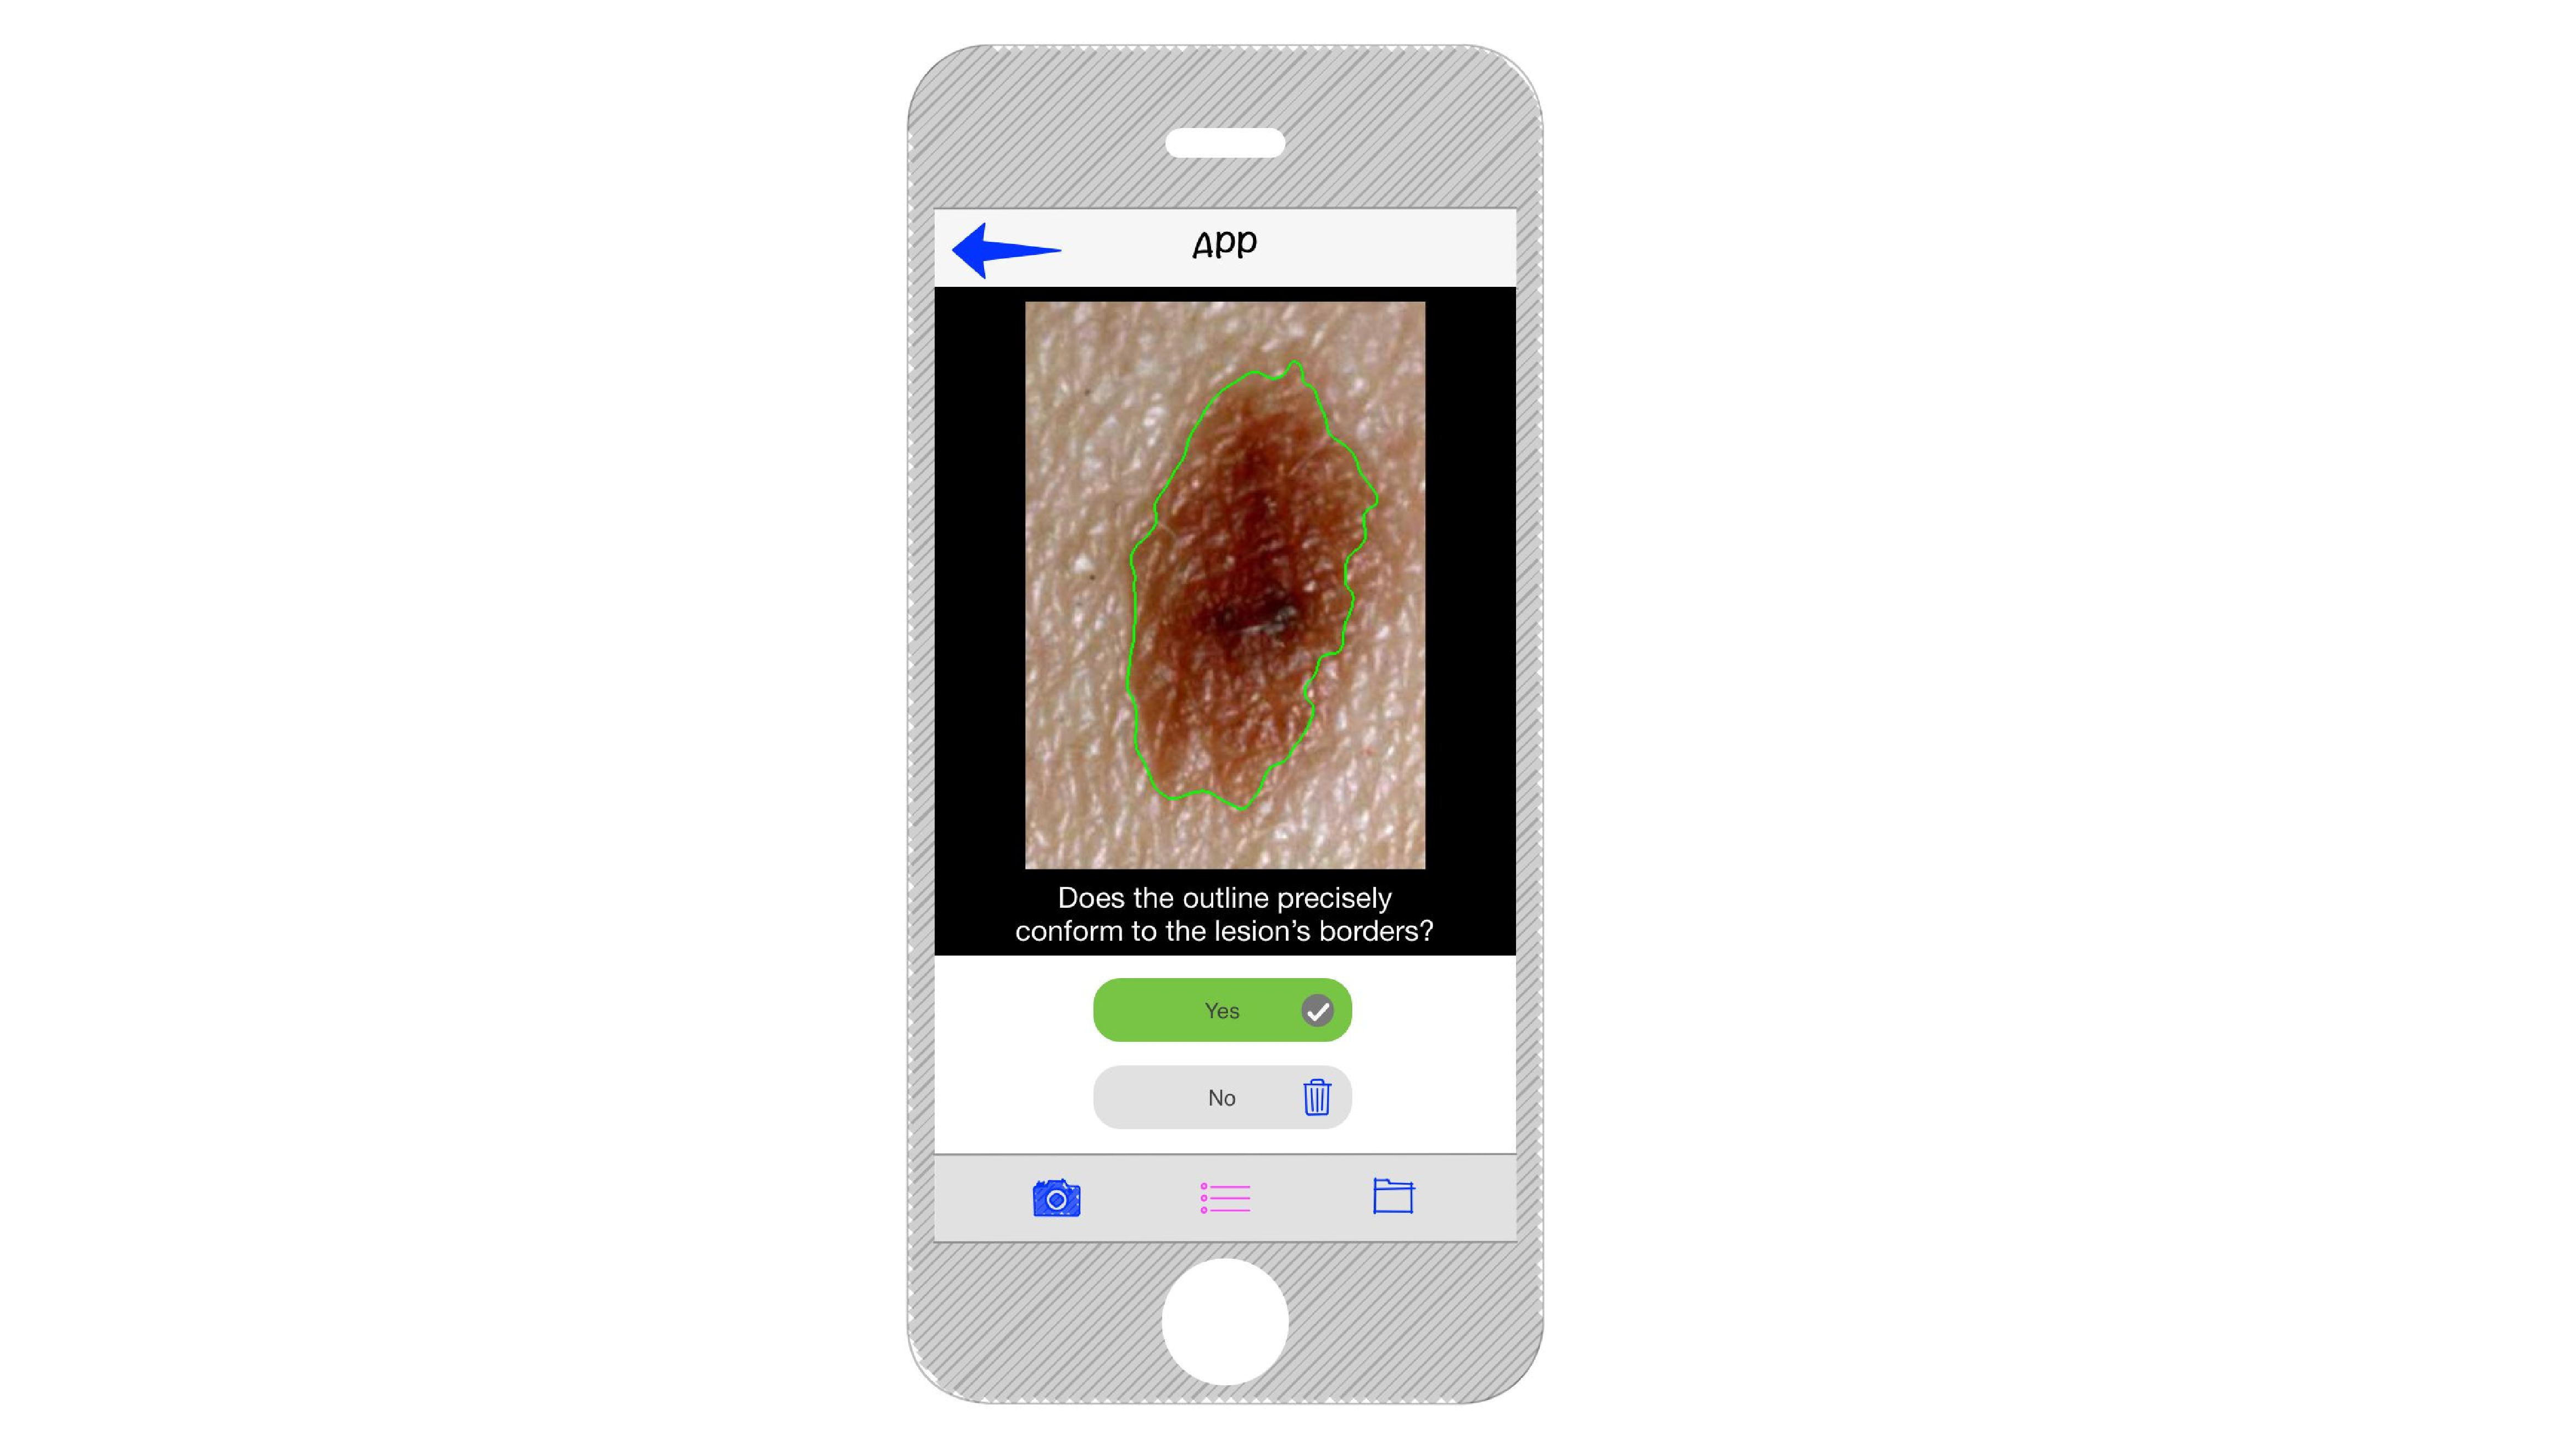
\includegraphics[height=10cm,keepaspectratio]{assets/GUI/border_confirm.pdf}
    \caption{Border Confirm View}
    \label{fig:border_confirm_view}
\end{figure}

\begin{figure}[H]
    \centering
    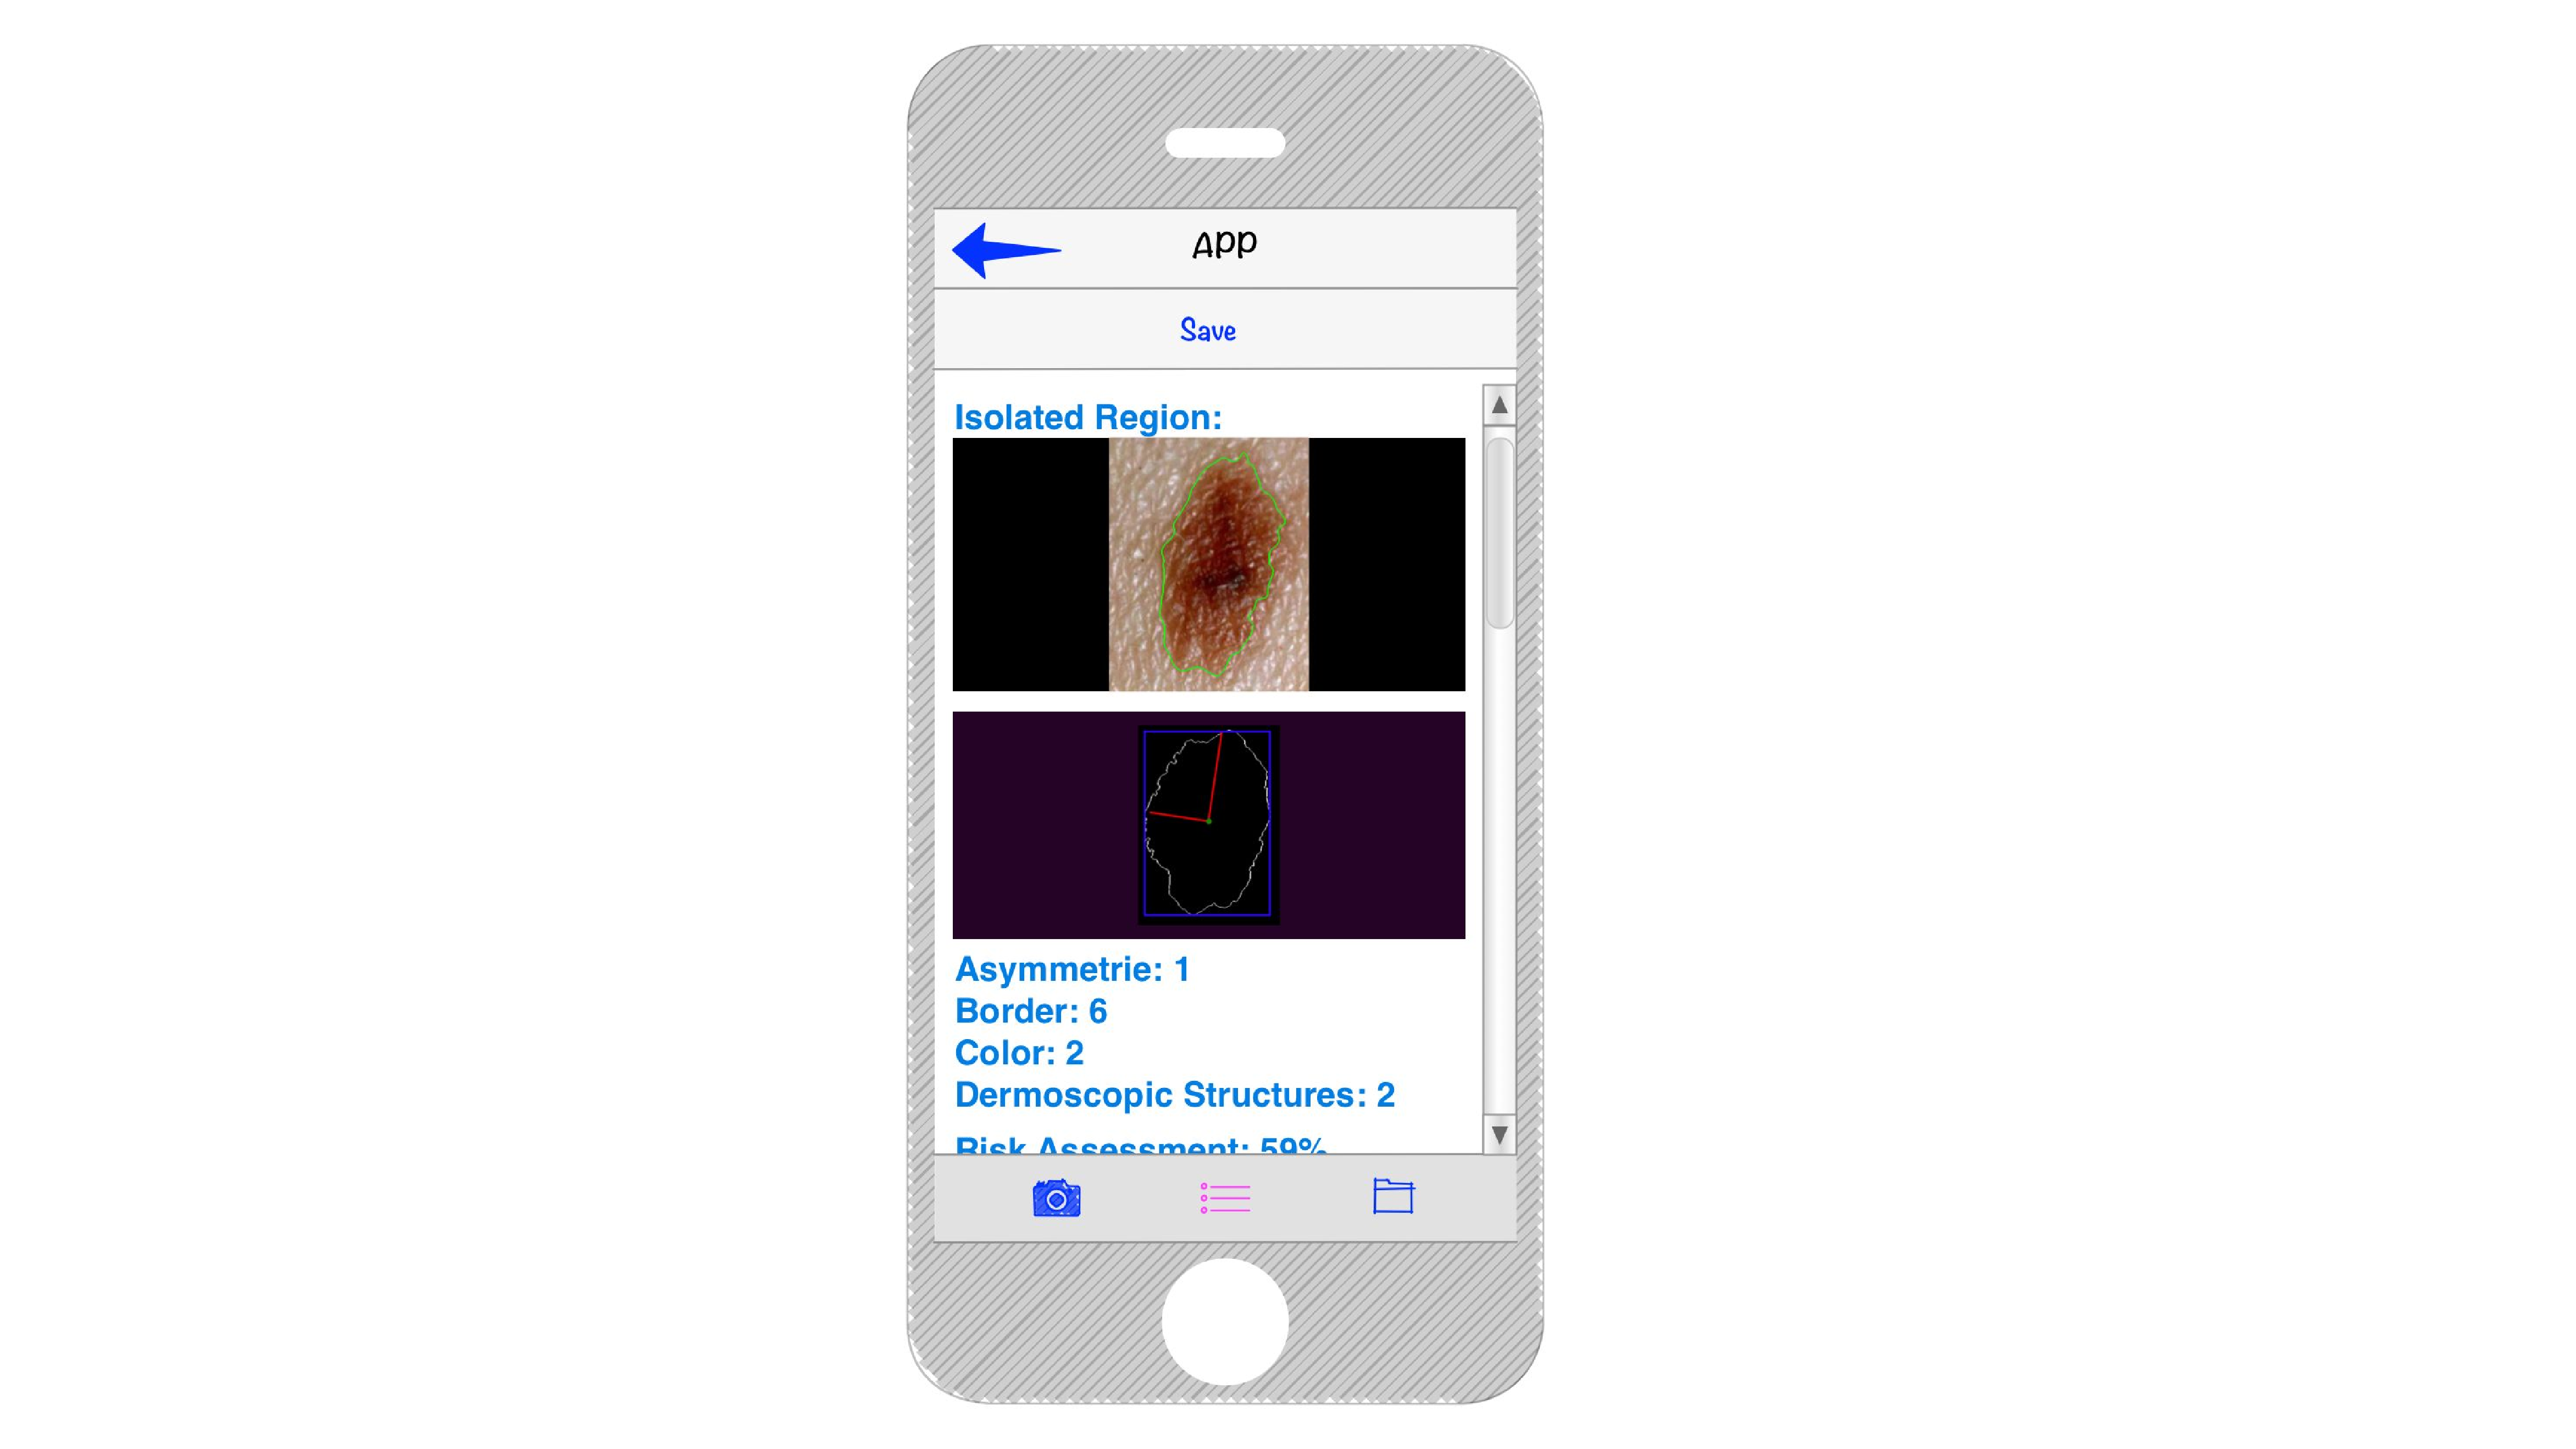
\includegraphics[height=10cm,keepaspectratio]{assets/GUI/image_detail_view.pdf}
    \caption{Image Detail View}
    \label{fig:image_detail_view}
\end{figure}

\begin{figure}[H]
    \centering
    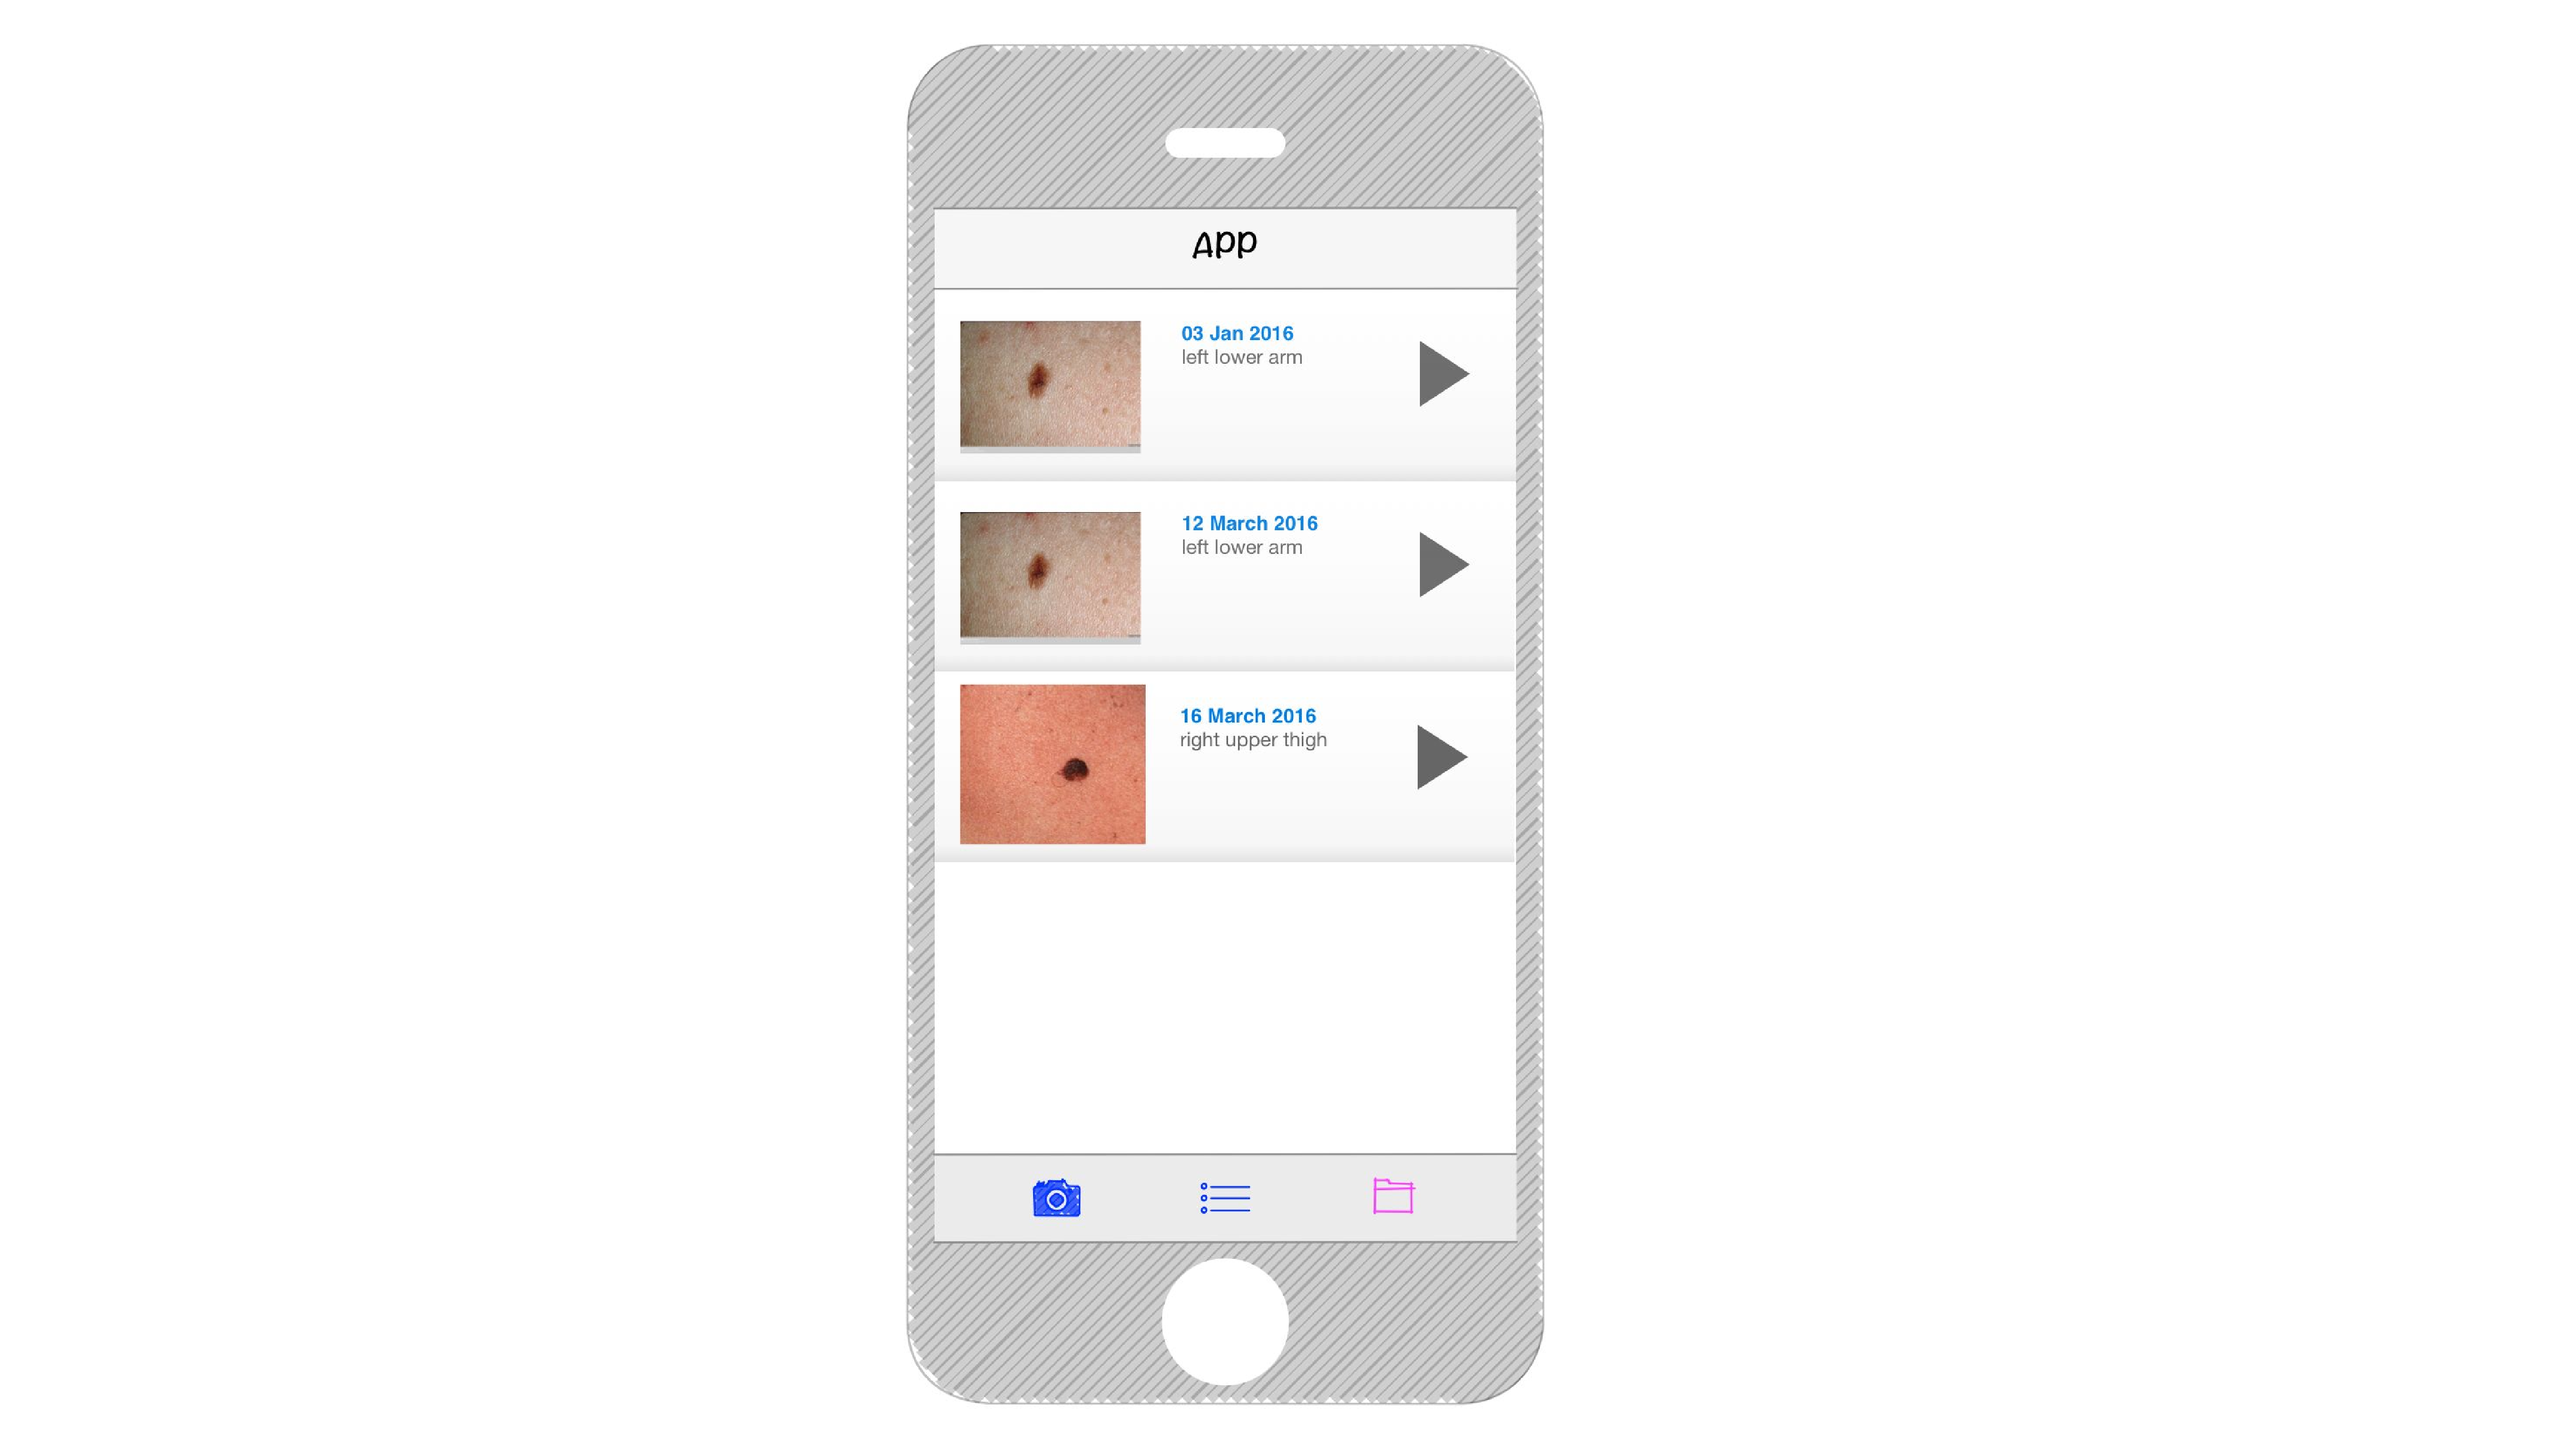
\includegraphics[height=10cm,keepaspectratio]{assets/GUI/archive_view.pdf}
    \caption{Archive View}
    \label{fig:archive_view}
\end{figure}

\begin{figure}[H]
    \centering
    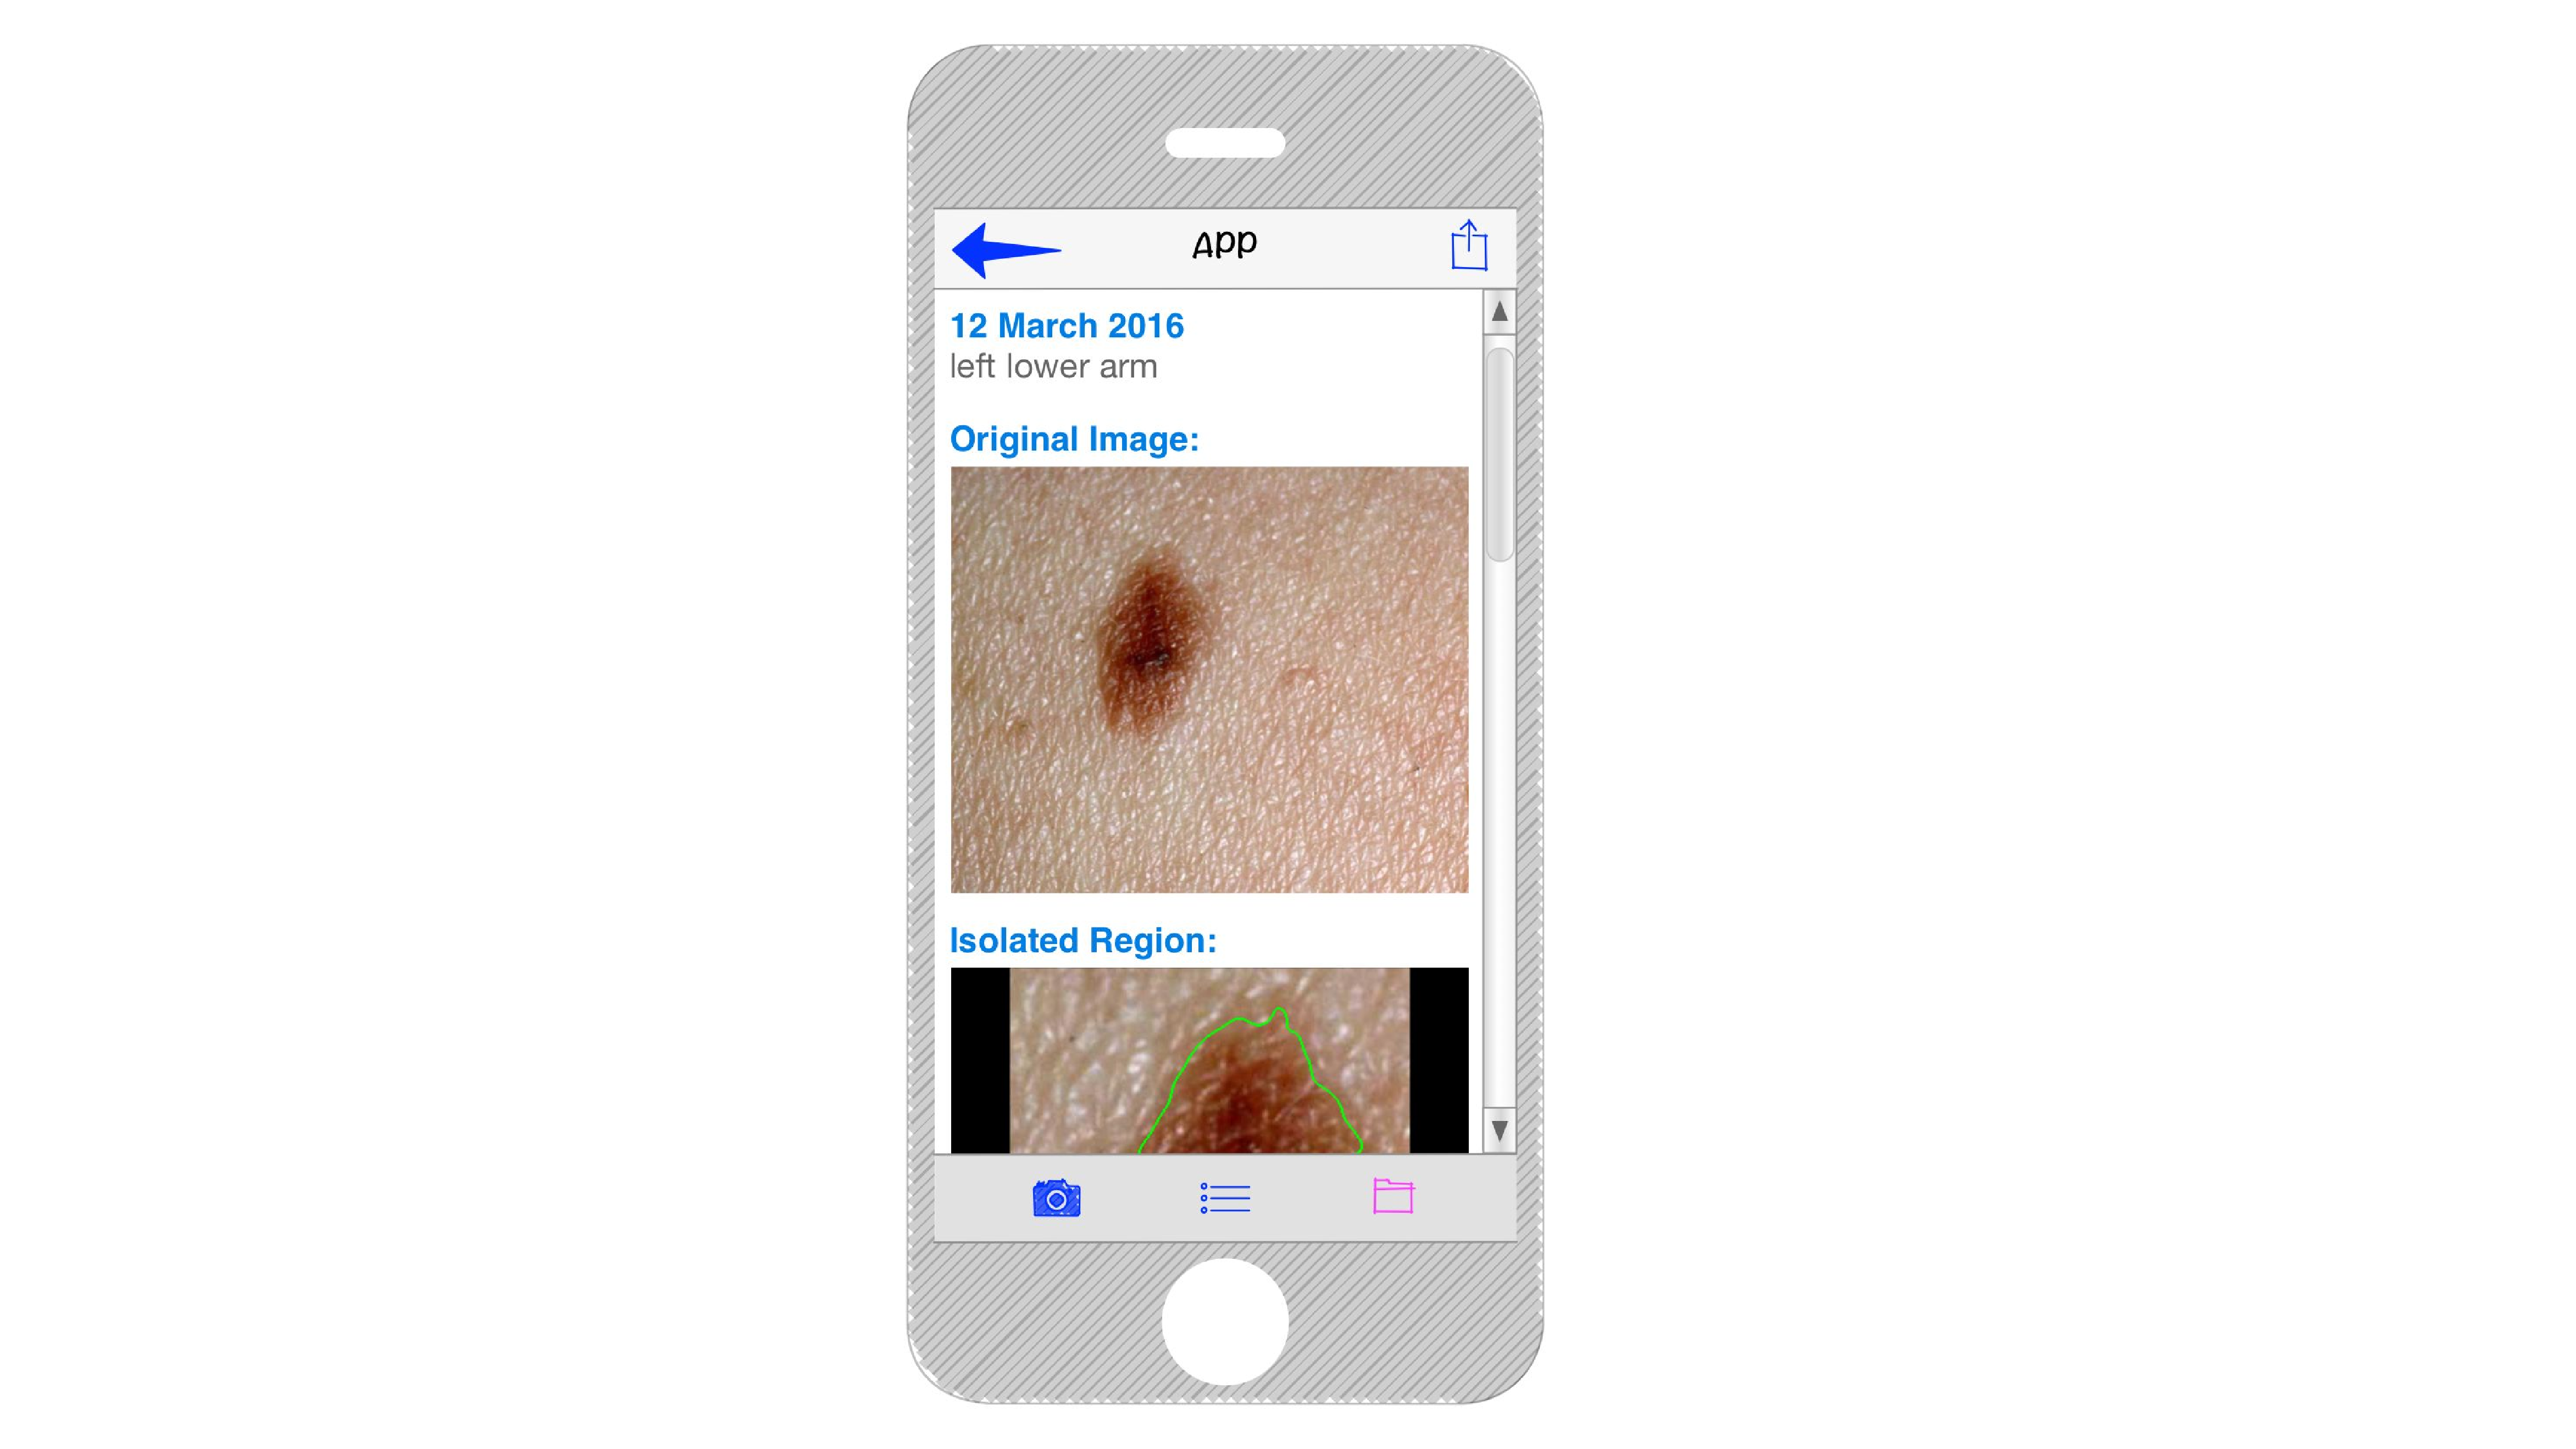
\includegraphics[height=10cm,keepaspectratio]{assets/GUI/archive_detail_view.pdf}
    \caption{Archive Detail View}
    \label{fig:archive_detail}
\end{figure}

\section{Requirements}

\section{Prioritized Requirements}

\begin{longtable}{ | l | l | l | l | l | l | l |}
\hline
ID & Priority & Name & Implemented  \\ \hline

REQ-F-1 & - & Preview Camera Input & -  \\ \hline
REQ-F-2 & - & Capture Camera Input & -  \\ \hline
REQ-F-3 & - & Border Extraction & -  \\ \hline
REQ-F-4 & - & Browse Images and Results & -  \\ \hline
REQ-F-5 & - & Select Image To View in Detail & -  \\ \hline
REQ-F-6 & - & Border Confirmation & -  \\ \hline
REQ-F-7 & - & Feature Extraction & -  \\ \hline
REQ-F-8 & - & Feature Extraction & -  \\ \hline


\caption{Prioritzed Requirement List}
\label{fig:prio_req}
\end{longtable}

\begin{table}[H]
    \begin{tabular}[t]{ | >{\bfseries}l | p{9.5cm} |}

    \hline
    ID
    &  REQ-F-1 \\ \hline

    Name
    & Preview Camera Input \\ \hline

    Description
    &  The system will let the user view a preview of the camera's input in realtime \\ \hline

    Preconditions
    & None \\ \hline

    Acceptance Tests
    & \\ \hline

    Relations
    & UC-1 \\ \hline

    Comments
    &  \\ \hline

    \end{tabular}

    \caption{Functional Requirement 1}
    \label{fig:req_f_1}

\end{table}
\begin{table}[H]
    \begin{tabular}[t]{ | >{\bfseries}l | p{9.5cm} |}

    \hline
    ID
    &  REQ-F-2 \\ \hline

    Name
    & Capture Camera Input \\ \hline

    Description
    &  The system will let the user capture an image from the camera's input. \\ \hline

    Preconditions
    & None \\ \hline

    Acceptance Tests
    & \\ \hline

    Relations
    & UC-1 \\ \hline

    Comments
    &  \\ \hline

    \end{tabular}

    \caption{Functional Requirement 2}
    \label{fig:req_f_2}

\end{table}
\begin{table}[H]
    \begin{tabular}[t]{ | >{\bfseries}l | p{9.5cm} |}

    \hline
    ID
    &  REQ-F-3 \\ \hline

    Name
    & Border Extraction \\ \hline

    Description
    &  The system must be able to calculate the border of a lesion in a captured image. \\ \hline

    Preconditions
    & None \\ \hline

    Acceptance Tests
    & \\ \hline

    Relations
    & UC-2 \\ \hline

    Comments
    &  \\ \hline

    \end{tabular}

    \caption{Functional Requirement 3}
    \label{fig:req_f_3}

\end{table}
\begin{table}[H]
    \begin{tabular}[t]{ | >{\bfseries}l | p{9.5cm} |}

    \hline
    ID
    &  REQ-F-4 \\ \hline

    Name
    & Browse Images and Results \\ \hline

    Description
    &  The system will let the user browse through a list of images. The list will display the status of the images. \\ \hline

    Preconditions
    & None \\ \hline

    Acceptance Tests
    & \\ \hline

    Relations
    &  \\ \hline

    Comments
    &  \\ \hline

    \end{tabular}

    \caption{Functional Requirement 4}
    \label{fig:req_f_4}

\end{table}
\begin{table}[H]
    \begin{tabular}[t]{ | >{\bfseries}l | p{9.5cm} |}

    \hline
    ID
    &  REQ-F-5 \\ \hline

    Name
    & Select Image To View in Detail \\ \hline

    Description
    &  The system will let the user select and view an image as well as the results of completed processes. \\ \hline

    Preconditions
    & None \\ \hline

    Acceptance Tests
    & \\ \hline

    Relations
    &  \\ \hline

    Comments
    &  \\ \hline

    \end{tabular}

    \caption{Functional Requirement 5}
    \label{fig:req_f_5}

\end{table}
\begin{table}[H]
    \begin{tabular}[t]{ | >{\bfseries}l | p{9.5cm} |}

    \hline
    ID
    &  REQ-F-6 \\ \hline

    Name
    & Border Confirmation \\ \hline

    Description
    & The system will let the user confirm that the border of a lesion hat been precisely calculated. \\ \hline

    Preconditions
    &  \\ \hline

    Acceptance Tests
    & \\ \hline

    Relations
    &  \\ \hline

    Comments
    &  \\ \hline

    \end{tabular}

    \caption{Functional Requirement 6}
    \label{fig:req_f_6}

\end{table}
\begin{table}[H]
    \begin{tabular}[t]{ | >{\bfseries}l | p{9.5cm} |}

    \hline
    ID
    &  REQ-F-7 \\ \hline

    Name
    & Feature Extraction \\ \hline

    Description
    & The system must be able to extract relavent features from the isolated lesion image. \\ \hline

    Preconditions
    &  \\ \hline

    Acceptance Tests
    & \\ \hline

    Relations
    &  \\ \hline

    Comments
    &  \\ \hline

    \end{tabular}

    \caption{Functional Requirement 7}
    \label{fig:req_f_7}

\end{table}
\begin{table}[H]
    \begin{tabular}[t]{ | >{\bfseries}l | p{9.5cm} |}

    \hline
    ID
    &  REQ-F-8 \\ \hline

    Name
    & Add To Process Queue \\ \hline

    Description
    & The system must be able to add an image process job to the process queue \\ \hline

    Preconditions
    &  \\ \hline

    Acceptance Tests
    & \\ \hline

    Relations
    &  \\ \hline

    Comments
    &  \\ \hline

    \end{tabular}

    \caption{Functional Requirement 8}
    \label{fig:req_f_8}

\end{table}
\begin{table}[H]
    \begin{tabular}[t]{ | >{\bfseries}l | p{9.5cm} |}

    \hline
    ID
    &  REQ-F-9 \\ \hline

    Name
    & Add/Save/Edit Metadata to Image and Results \\ \hline

    Description
    & The system will allow the user to add or edit metadata associated with the captured image. \\ \hline

    Preconditions
    &  \\ \hline

    Acceptance Tests
    & \\ \hline

    Relations
    &  \\ \hline

    Comments &
        The metadata associated might include the date when the image was captures as well as the location on the body where the lesion is located. The metadata will have the form of a text input field where the user can enter any text. It could be extended, if necessary, with structured data fields.

    \\ \hline

    \end{tabular}

    \caption{Functional Requirement 9}
    \label{fig:req_f_9}

\end{table}
\begin{table}[H]
    \begin{tabular}[t]{ | >{\bfseries}l | p{9.5cm} |}

    \hline
    ID
    &  REQ-F-10 \\ \hline

    Name
    & Save Image and Associated Data as Archive. \\ \hline

    Description
    & The system will allow the user to save images and associated data for reassessment and comparison in the future. \\ \hline

    Preconditions
    &  \\ \hline

    Acceptance Tests
    & \\ \hline

    Relations
    &  \\ \hline

    Comments &

        Storage on a mobile device is a limited resource. Depending on the development strategy chosen, Web App vs Native, the application might not have access to it's own data store. It would be useful to offload data to a cloud or web based storage location.

    \\ \hline

    \end{tabular}

    \caption{Functional Requirement 10}
    \label{fig:req_f_10}

\end{table}
\begin{table}[H]
    \begin{tabular}[t]{ | >{\bfseries}l | p{9.5cm} |}

    \hline
    ID
    &  REQ-F-11 \\ \hline

    Name
    & Browse Images and Results from Archive. \\ \hline

    Description
    & The sytem will allow the user to browse previously saved images and results from the archive. \\ \hline

    Preconditions
    &  \\ \hline

    Acceptance Tests
    & \\ \hline

    Relations
    &  \\ \hline

    Comments
    &  \\ \hline

    \end{tabular}

    \caption{Functional Requirement 11}
    \label{fig:req_f_11}

\end{table}

\section{Prioritisation}
This project will employ a Single-Criterion Ad-hoc prioritisation classification as opposed to an analytical approach such as the Wiegers prioritisation matrix. The rationale behind this choice is that as a single person development project the determination of weights for benefit, detriment, cost, and risk is an ad-hoc exercise. In a larger project with multiple developers and active stakeholders the time and effort required for a prioritisation assessment according to Wiegers would be advisable.

The following are the prioritisation classes as defined in \cite{9781937538774}:

\begin{itemize}[label={}]

\item \textbf{Mandatory}: A mandatory requirement is a requirement that must be implemented at all costs or else the success of the system is threatened.
\item \textbf{Optional}: An optional requirement is a requirement that does not necessarily need to be implemented. Neglecting a few requirements of this class does not threaten the success of the system.
\item \textbf{Nice-to-have}: Nice-to-have requirements are requirements that do not influence the system’s success if they are not implemented.

\end{itemize}



\section{Software Architecture}
\subsection{MVC}
Since the 1970s the Model View Controller ( MVC ) pattern is the standard architectural design pattern for applications that present the user with a graphical user interface. It was developed out of a need for modularity, to encapsulate responsibility of specific concepts to separate program modules, or Separation of Concerns. MVC identifies three main components that program code should be grouped into, namely\cite{walther_2016}:

\begin{itemize}[label={}]

\item \textbf{Model}: The representation of some object of knowledge, encapsulates code managing the associated data and behaviour ( business-logic ).
\item \textbf{View}: The visual representation of the model. The view can feature or hide aspects of the model and thus act as a presentation filter. The view observe the model for changes and update the presentation accordingly.
\item \textbf{Controller}: The controller allows the user to interact with the model. It allows the user to trigger behaviours implemented in the Model.

\end{itemize}

In the classic MVC pattern the model does not "know" about the view or the controller. And the controller does not effect the view. Instead, both the view and controller monitor the model using an observer mechanism and synchronise themselves when updates to the model occur.

\begin{figure}[H]
    \centering
    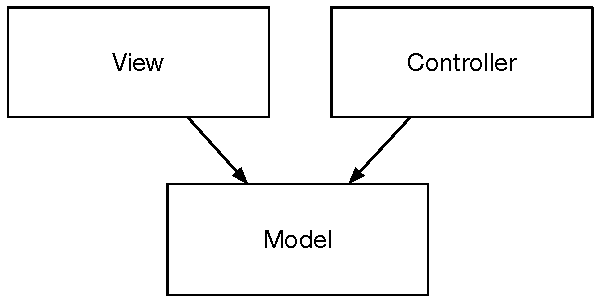
\includegraphics[height=4cm,keepaspectratio]{assets/concept/mvc_1.pdf}
    \caption{Classic MVC}
    \label{fig:mvc_1}
\end{figure}

\subsection{Modern MVC}

Modern MVC has evolved from being a software design pattern which handles components of an application to an architectural design pattern that defines the structure of an application itself. It has many similarities to the Layer Architecture. The responsibilities of each layer are slightly different to the typical presentation, business, and persistence layer definitions.

Most modern web frameworks such as Ruby on Rails, Symfony or the IOS environment refer to themselves as MVC based frameworks. The modern MVC concept has changed slightly. The component definitions are the same, but some responsibilities have shifted. Modern MVC strictly separates the model from the view. All modern frameworks state that the view should have as little logic as possible. Any logic implemented in the view should only be relevant to presentation. The view components should not directly reference the model components\cite{apple_MVC}\cite{symfony_MVC}.

\begin{figure}[H]
    \centering
    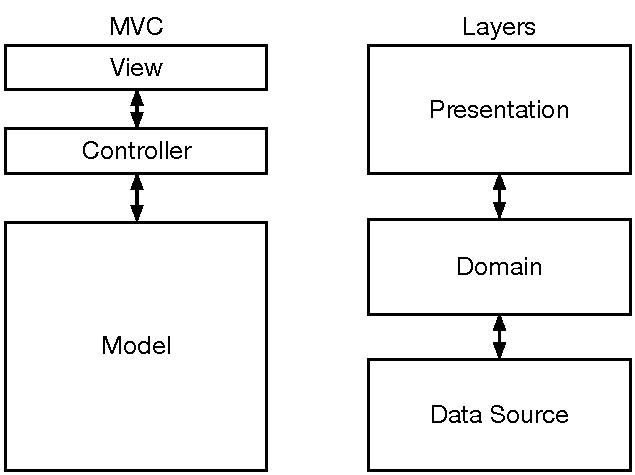
\includegraphics[height=4cm,keepaspectratio]{assets/concept/mvc_2.pdf}
    \caption{Modern MVC vs 3-Tier Layered Architecture}
    \label{fig:mvc_2}
\end{figure}

This division of responsibility has the added benefit of increased testability. GUIs are difficult to test, by removing as much logic as possible from the user interface there is less necessity to test it. The controller and model components can more easily be tested independently of one another using normal unit tests\cite{mvp_testing}.

\subsection{MVC Derivatives}

Many MVC derivatives exist. The main differences are where the division of responsibility is made and how it is labeled. MVVM defines a view model instead of a controller. The view model acts as a facade around the model and introduces a data binder element that is responsible for keeping the view and view model synchronised. The MVT, calls the view a template and the controller a view. The slight difference is that the template is basically a static file, with no logic, and placeholders for the data. The Django web framework uses this model, but there is little difference to the other MVC derivatives such as MVP ( model view presenter ). The AngularJS web framework takes ends the discussion of which design to follow by labelling itself a MVW ( model view whatever ) framework\cite{mvw}.


\begin{figure}[H]
    \centering
    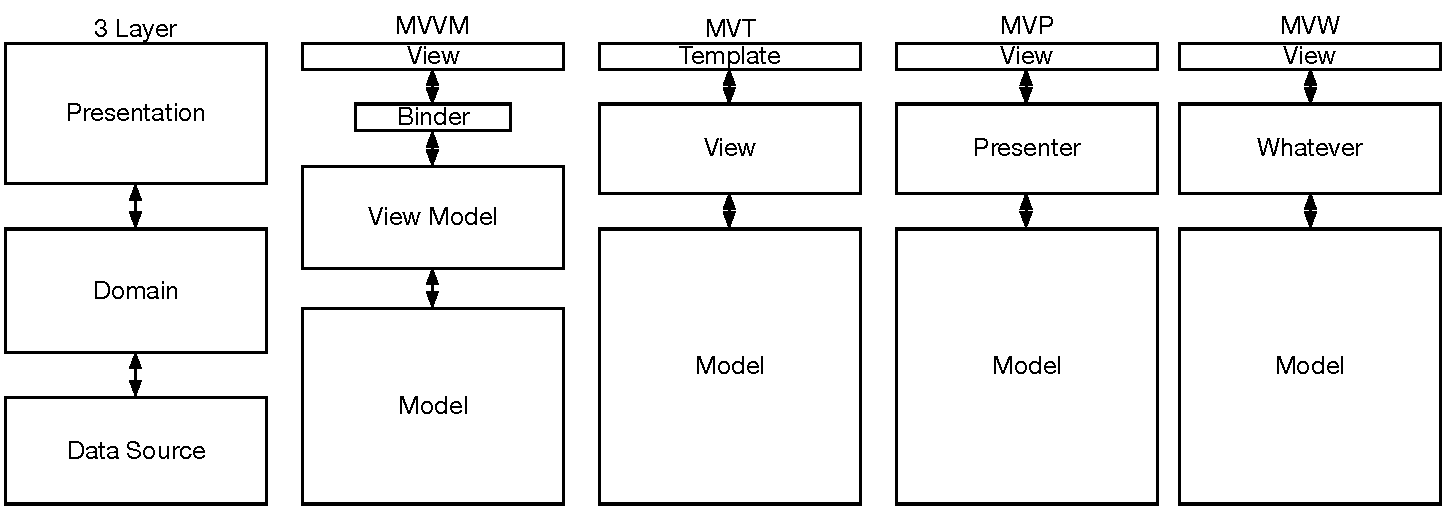
\includegraphics[height=4cm,keepaspectratio]{assets/concept/mvc_3.pdf}
    \caption{MVC Derivatives Overview}
    \label{fig:mvc_alt}
\end{figure}

\subsection{MVC and Smart Phone Applications}

Although most frameworks and environments targeted toward mobile application development use concepts from MVC, it can be difficult to define strict devision of responsibility, especially in conjunction with services provided from an online server. Often the responsibilities of the controller are reimplemented server side, some model management might occur in the app. Server and application code are developed using different languages and often most likely different developers. One solution is is to develop the app as a thin client, where it basically becomes the view component of MVC and the controllers and model are implemented on the server. Taken to the extreme, the app runs in a standard web browser and server provides the view components that emulate a native mobile user interface. This is referred to as a web app. Any logic in the view is implemented using javascript. Hardware support is limited to what the mobile browser provides access to. In order to extend hardware support a hybrid approach can be used in which the app implements a custom browser view which is extended with native capabilities. Here is division or responsibilities as defined by MVC become fuzzy. A fully native app working in conjunction with a web server will not conform well to the definitions of MVC.

\subsection{VIPER}

VIPER is a new software architecture pattern which extends MVC with some addition concepts that make it more adaptable to mobile applications, especially when they are extended with online server based services. The classic controller is split into a presenter and a controller, the model component is split into a central data manager communicating with many services and entities\cite{viper}.

\begin{figure}[H]
    \centering
    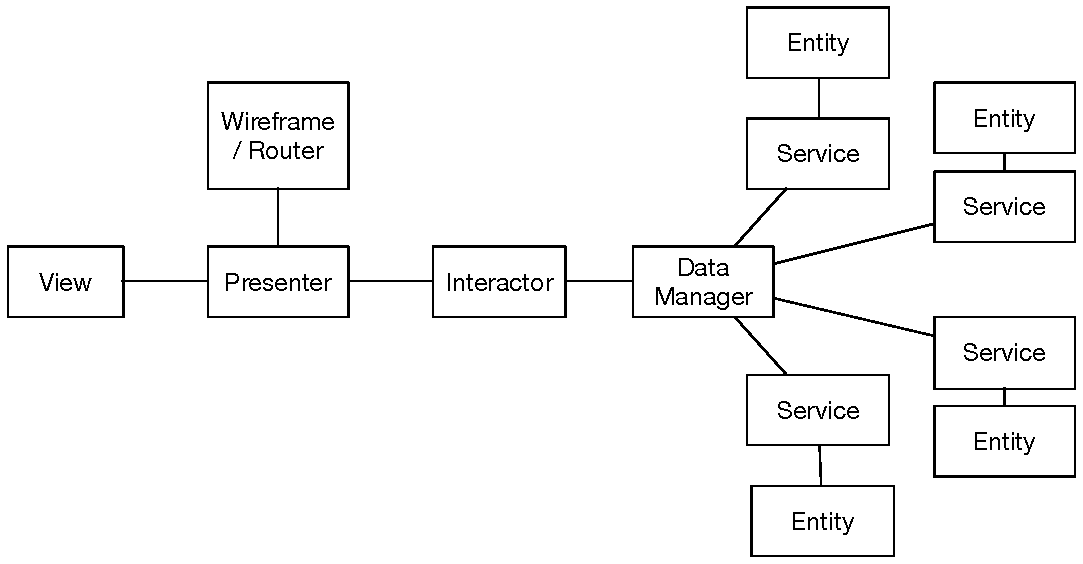
\includegraphics[height=6cm,keepaspectratio]{assets/concept/viper.pdf}
    \caption{VIPER Overview}
    \label{fig:viper}
\end{figure}

\begin{itemize}[label={}]

\item \textbf{View}: The view corresponds to the view as defined in modern MVC definitions, it is a slim component with as little logic as possible. It presents the current state of the models and provides “widgets” with which the user can interact.
\item \textbf{Presenter}: The presenter passes data to the view and handles events from the view. The presenter might perform some basic validation, in the case of a user sign-up scenario, for example, the presenter might validate that a user’s email is indeed formatted as a correct email, it will not validate if the email has already been used by someone else.

\item \textbf{Interactor}: Business logic is handled by the interactor. Most a what the model component in MVC was responsible for is handled here. The interactor however does not know anything about data storage, databases, or persistence. It does not know if data is local or accessible via a network.

\item \textbf{Data Manager}:
\item \textbf{Service}:
\item \textbf{Entity}:
\item \textbf{Wireframe / Router}:

\end{itemize}
